\capitulo{4}{Técnicas, herramientas y componentes}

Durante el proyecto se han utilizado diferentes tecnologías, herramientas y componentes que son imprescindibles y necesitan conocerse antes de continuar con el proyecto. Para optar por éstos y no por otros, se ha realizado una valoración que queda plasmada en este apartado a modo de justificación.

\section{Entorno Software}
\subsection{Raspbian (Distribución Linux)}\label{4:RaspbianOS}
Como he comentado anteriormente, pretendo correr una distribución Linux en nuestro microPC. Las placas Raspberry Pi disponen de unas distribuciones de Linux desarrolladas expresamente para su hardware desde la Raspberry Pi Foundation. De esta manera conseguimos que el entorno esté diseñado para el hardware donde será ejecutado incluyendo, además, utilidades preinstaladas para explotarlas más fácil y eficientemente. Una de estas distribuciones optimizadas y orientadas a estas placas es Raspbian~\cite{misc:RbPWeb} o Raspberry Pi OS, que incluye software orientado a la educación, programación y otras de uso general. Algunas de estas aplicaciones son Python~\cite{misc:Python} (Lenguaje de programación que pretende que se desarrolle cógigo de una forma sencilla, rápida, poco costosa y legible), Scratch~\cite{misc:Scratch}(Simulador amigable para aprender programación.) o Java\cite{misc:Java}(Lenguaje de programación multiplataforma que utiliza una máquina virtual transparente para el usuario para ejecutarse), entre otros.

\subsection{Entorno de desarrollo Bash}\label{4:BASH}
\begin{itemize}
    \item \textbf{Herramientas valoradas:} \href{https://www.freebsd.org/cgi/man.cgi?query=vi&sektion=1}{Vi},~\href{https://www.vim.org/}{Vim}, \href{https://www.nano-editor.org/}{Nano}.
    \item \textbf{Herramienta elegida:} \href{https://www.nano-editor.org/}{Nano}.
\end{itemize}

Nuestro Sistema Operativo Raspbian\cite{misc:RbPWeb}, al ser una distribución de Linux~\cite{misc:Linux}, dispone de líneas de comandos, procesadores de texto plano y editores de texto integrados. Éste es un editor de textos básico que facilita la interacción con él pese a que Vi o Vim son mucho más potentes.

\subsection{Entorno de desarrollo Python}\label{4:Python}
\begin{itemize}
    \item \textbf{Herramientas valoradas:} \href{https://www.jetbrains.com/es-es/pycharm/}{Jetbrains PyCharm} y \href{https://jupyter.org/}{Jupyter Notebook}.
    \item \textbf{Herramienta elegida:} \href{https://jupyter.org/}{Jupyter Notebook}.
\end{itemize}

Jupyter Notebook es un entorno de desarrollo interactivo y open source, basado en cuadernos que estructuran el código pudiendo ejecutarlo todo o parte. Dispone de una interfaz limpia, ligera e interactiva que nos permite programar en 40 lenguajes, incluyendo Python~\cite{misc:Python}.

\section{Control de datos}
\subsection{Web Scraping}\label{4:WebScraping}
Es una técnica utilizada para extraer información de una página web utilizando las etiquetas de que dispone el propio lenguaje interpretado de HTML (del inglés <<HyperText Markup Language>> o lenguaje de marcas de hipertexto) para organizar elementos dentro de una página web, de forma que se introduce dentro de una etiqueta y subetiquetas hasta llegar al contenido del elemento requerido. Podemos entenderlo como si fueran contenedores lógicos configurables.
En nuestro caso, podremos utilizarlo desde Python~\cite{misc:Python} sirviéndonos de la librería <<beautifulsoup>> siempre que necesitemos obtener información de una página web.

\subsection{APIS}\label{4:APIS}
\begin{itemize}
    \item \textbf{API situación geográfica}
\end{itemize}
En primer lugar estuve haciendo pruebas con la API de \url{www.ifconfig.me/ip} que devuelve la provincia en la que se encuentra tu IP pública pero quería una información más precisa ya que no tendremos la misma temperatura en El Escorial que en Aranjuez. Por ello, opté por \url{http://ip-api.com} que sí obtiene correctamente la ciudad desde la que nos conectamos.

\begin{figure}
    \centering
    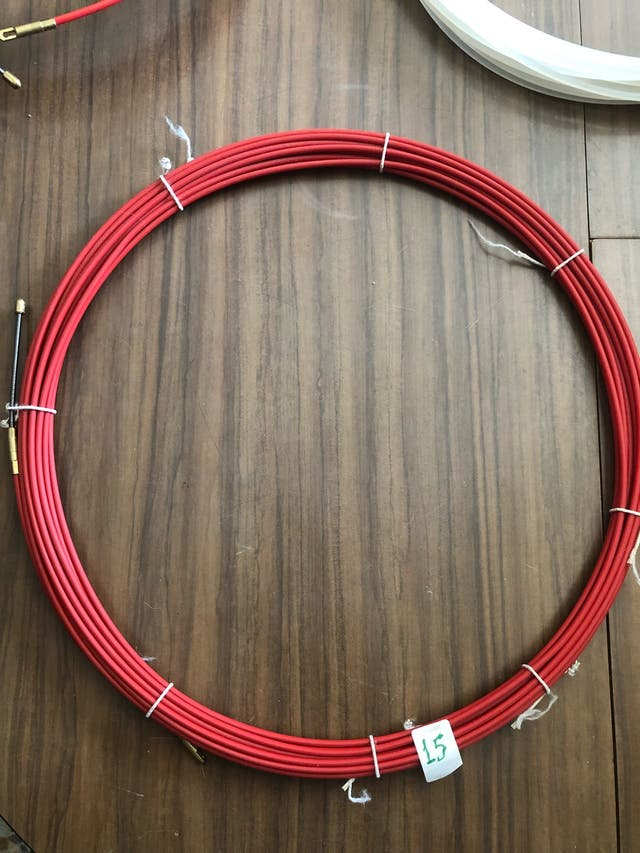
\includegraphics[width=0.6\textwidth, angle=90]{img/fotos/guiaPasacables.jpg}
    \caption{Guía pasacables.} \label{Img:guiaPasacables}
\end{figure}

\begin{itemize}
    \item \textbf{API Tiempo}\label{4:API_Tiempo}
\end{itemize}
Al principio probé la API de \url{www.weatherapi.com} pero me entregaba únicamente la hora de salida y puesta del sol, lo cual es correcto para el control básico de las persianas pero quería llevar el proyecto más allá obteniendo además, una previsión de las temperaturas para el día siguiente pudiendo trabajar con ésta haciendo gráficos y poder decidir si encenderemos la calefacción o no. Y, por ello, opté por probar con la API de \url{www.climacell.co} que además, aseguran que es un 60\% más fiable que otras APIS ya que obtiene información de teléfonos móviles, cámaras y otros servicios online.

\subsection{json}\label{4:JSON}
La librería json~\cite{misc:Json} para Python~\cite{misc:Python} y Python v3 nos permite, entre otros, parsear el código json~\cite{misc:Json} de archivos mediante la estructura de \textit{key:value}. En nuestro caso, tras obtener información de las APIs trataremos dicha información como json~\cite{misc:Json} gracias a su librería para Python~\cite{misc:Python}.

\section{Técnicas manuales}

\subsection{Tirada de cable con guía pasacables}\label{4:guiaPasacables}
Podemos ver una guía pasacables en la imagen~\ref{Img:guiaPasacables}~\footnote{Imagen Original de www.wallapop.es}.
El procedimiento a seguir es el siguiente:
\begin{enumerate}
        \item Se abren las tapas de dos cajas de derivación próximas.
        \item Se introduce una guía pasacables (herramienta plástica con la forma de cuerda para introducir cables por canalizaciones) por el extremo de uno de los tubos dentro de la caja hasta llegar al otro extremo.
        \item Se asegura el cable a uno de los extremos de la guía pasacables.
        \item Se tira del otro extremo de la guía pasacables hasta conseguir sacar el cable por éste.
\end{enumerate}





\section{Metodologías}
\subsection{Scrum}\label{4:SCRUM}
Scrum\cite{manual:Scrum} es un marco de trabajo para el desarrollo de software mediante la metodología ágil en el que se busca realizar un trabajo colaborativo de desarrollo incremental. Se aplica una metodología basada en milestones y sprints de forma iterativa.

\subsection{Modularidad}\label{4:Modularidad}
Utilizaremos la modularidad para subdividir la aplicación en pequeños subprogramas que tienen una pequeña funcionalidad. De esta manera es más fácil detectar errores y escalar el proyecto. Además, teniendo clara la entrada y salida de cada uno de los módulos se pueden lanzar pruebas a cada uno de los módulos para comprobar su correcto funcionamiento mejorando, también, el mantenimiento.

\section{Entorno de desarrollo del Proyecto}

\subsection{Control de versiones o CVS, Concurrent Versioning System}\label{4:controlVersiones}
\begin{itemize}
    \item \textbf{Herramientas valoradas:} \href{https://git-scm.com/}{Git}, \href{https://subversion.apache.org/}{SVN}.
    \item \textbf{Herramienta elegida:} \href{https://git-scm.com/}{Git}.
\end{itemize}

Git es un software destinado al control de versiones software en el que se registran los cambios producidos en el mismo, facilitando la integración de código por parte de cualquiera de los integrantes del proyecto.
La diferencia más notable entre ellos es que Git es distribuido y SVN es un sistema centralizado. Significa que Git nos permite disponer de una copia en cada uno de los equipos desde los que se trabaje haciendo un clonado del repositorio, mientras que en SVN también permite el trabajo directamente en la nube.

\subsection{Hosting del Repositorio}\label{4:GitHUb}
\begin{itemize}
    \item \textbf{Herramientas valoradas:} \href{https://github.com/}{Github} y \href{https://bitbucket.org/product/}{Bitbucket}.
    \item \textbf{Herramienta elegida:} \href{https://github.com/}{Github}.
\end{itemize}

Ambas opciones de hosting de repositorios funcionan de forma similar aunque GitHub incorpora opciones como la revisión de código, Kanban, Wikis o tableros entre otros que me han hecho decantarme por esta opción.
Ésta, es la plataforma principal de trabajo, que a su vez es una red social de código donde cualquiera puede contribuir en proyectos públicos y Open Source.


\subsection{Gestión del proyecto}\label{4:ZenHub}
\begin{itemize}
    \item \textbf{Herramientas valoradas:} \href{https://teams.microsoft.com/}{MS.Teams}, \href{https://www.zenhub.com/}{ZenHub}, \href{https://github.com/}{GitHub Projects}, \href{https://www.zenhub.com/}{Trello}, \href{https://www.atlassian.com/es/software/jira}{Jira}, \href{https://www.board.com/es#gref}{Board}, \href{https://monday.com/lang/es/}{Monday}, \href{https://zube.io/}{Zube}, \href{https://clubhouse.io/}{Clubhouse}.
    \item \textbf{Herramienta elegida:} \href{https://www.zenhub.com/}{ZenHub}.
\end{itemize}

Es la única solución de colaboración en equipo integrada en GitHub y nos permite planificar hojas de ruta, generar informes, gestionar con Kanban, gestión ágil del proyecto mostrando la situación del proyecto para conseguir aumentar la productividad del equipo.

\subsection{Editor del proyecto}\label{4:ATOM}
\begin{itemize}
    \item \textbf{Herramientas valoradas:} \href{https://atom.io/}{Atom}, \href{https://code.visualstudio.com/}{Visual Studio Code}, \href{https://www.sublimetext.com/}{Sublime}.
    \item \textbf{Herramienta elegida:} \href{https://atom.io/}{Atom}.
\end{itemize}

Es un editor de código y texto creado por GitHub integrando las funciones de Git y GitHub, lo que nos facilita trabajar en nuestro equipo y replicar los cambios en Git, GitHub y ZenHub. Además, es un software multiplataforma, licencia open source, completamente personalizable, con temas y múltiples plugins, autocompletado y fácil navegación.
En este proyecto se utilizará para publicar las actualizaciones del proyecto.



\subsection{Dibujos, diagramas y planos}\label{4:plataformasDibujosYPlanos}
\begin{itemize}
    \item \textbf{Herramientas valoradas:} \href{https://fritzing.org/}{Fritzing}, \href{https://support.microsoft.com/es-es/windows/obtener-microsoft-paint-a6b9578c-ed1c-5b09-0699-4ed8115f9aa9}{Paint, Paint3D}, \href{https://www.adobe.com/es/products/photoshop.html}{Photoshop}, y \href{www.draw.io}{Draw.io}.
    \item \textbf{Herramienta elegida:} \href{https://fritzing.org/}{Fritzing} y \href{www.draw.io}{Draw.io}.
\end{itemize}
Realmente no pude decidirme por entre Fritzing y draw.io puesto que cada uno está orientado a un tipo de tarea:

Fritzing es un software con licencia Open Source\cite{misc:OpenSource} que nos permite realizar material electrónico fácilmente, aunque desde hace algún tiempo debemos hacer un pequeño desembolso por la descarga. En mi caso con el fin de entregar diagramas de calidad los haré con este software.

Por otro lado, Draw.io está pensado para hacer planos y dibujos que no están orientados a la electrónica, por lo que es muy útil para hacer otro tipo de diagramas.

\subsection{Procesador de textos \LaTeX}\label{4:latex}
\begin{itemize}
    \item \textbf{Herramientas valoradas:} \href{https://www.latex-project.org/}{\LaTeX}, \href{https://www.microsoft.com/es-es/microsoft-365/word}{MS Word}, \href{https://www.sublimetext.com/}{Sublime}, \href{https://www.overleaf.com/}{Overleaf}.
    \item \textbf{Herramienta elegida:} \href{https://www.latex-project.org/}{\LaTeX} y \href{https://www.overleaf.com/}{Overleaf}.
\end{itemize}
\LaTeX{} es un editor de textos open source\cite{misc:OpenSource} con alta calidad tipográfica que trabaja con etiquetas permitiéndonos separar nuestro contenido del estilo del mismo. Para escribir el proyecto en \LaTeX utilizaré Overleaf por su capacidad de compilado instantáneo, de forma que se puede comprobar cómo modificas la redacción en cada compilado.

\section{Entorno físico}

En el mercado existen diversas opciones para poder generar un proyecto como este. Las opciones a considerar son los SBC y los MicroPc.
\begin{itemize}
    \item \textbf{SBC}: Son pequeños equipos de placa única de bajo coste. Es el grupo de componentes en el que podemos encontrar Raspberry Pi y Arduino.
    \item \textbf{MicroPc}: Son pequeños equipos con mayor potencia y un precio más elevado que los anteriores. En este grupo podemos encontrar soluciones como los ShuttlePC.
\end{itemize}

Entre estas dos opciones, optaremos por la primera por varios motivos. El motivo principal es el coste: es innecesario hacer mayor desembolso para implementar este sistema domótico. Otros motivos son el consumo, que es mucho menor en las placas SBC y la necesidad de una plataforma intermedia para poder controlar los relés, que también incrementaría el precio.

\subsection{Comparativa SOC}
Tras determinar la utilización de un SoC se hizo una comparativa entre las dos SBC principales, Arduino y Raspberry Pi teniendo en cuenta que son dos placas muy similares.

\subsubsection{RaspberryPi}\label{4:RaspberryPi}
Para dar un enfoque muy general, podemos decir que las placas RaspberryPi~\cite{misc:RbPWeb} son microordenadores que disponen de poca potencia si las comparamos con equipos usuales, pero disponen de suficiente potencia para llevar a cabo este tipo de proyectos.

Se diseñaron en su origen por la RaspBerry Pi Foundation~\cite{misc:RbPWeb} en el Reino Unido para dotar de equipos informáticos a los centros de estudios a un bajo coste, pero el proyecto ha evolucionado para poder desarrollar, además, otras muchas tareas como puede ser nuestro caso, que la utilizaremos como ‘núcleo’ de toda nuestra instalación domótica y, será donde configuremos todo el entorno domótico de la vivienda.
Estas placas pueden ejecutar con agilidad distribuciones Linux~\cite{misc:Linux}, y desde sus éstas, podemos interactuar con sus famosos <<GPIO>>~\cite{misc:descubrearduino} como explicamos en el punto \ref{concepto:GPIO}, ver imagen ~\ref{Img:Especificaciones RBP2B}~\footnote{Imagen original de ~\url{https://raspberryparatorpes.net/ }}.

Podemos ver en la tabla~\ref{tab:comp_RBP} una comparativa de los modelos B de Raspberry Pi. A modo de resumen, únicamente he representado los modelos B en al comparativa porque el proyecto se ha realizado con un modelo B.

\begin{landscape}
\begin{table}[]
\centering
\resizebox{1.6\textwidth}{!}{%
\begin{tabular}{|c|c|c|c|c|c|}
\hline
\rowcolor[HTML]{C0C0C0} 
\color[HTML]{333333} \textbf{Modelo Raspberry Pi} & \textbf{Zero y Zero W} & \textbf{B+} & \textbf{2B} & \textbf{3B y 3B+} & \textbf{4B} \\ \hline
\textbf{Precio(Amazon)}   & \href{https://www.amazon.es/Raspberry-Pi-Zero-wh/dp/B07BHMRTTY/}{29,30€}   & \href{https://www.amazon.es/Raspberry-Pi-Desktop-Tarjeta-Broadcom/dp/B00LPESRUK/}{34,30€} & \href{https://www.amazon.es/gp/product/B00T2U7R7I/}{51,59€} & \href{https://www.amazon.es/Raspberry-Pi-Modelo-Quad-Core-Cortex-A53/dp/B01CD5VC92/}{37,44€}  & \href{https://www.amazon.es/RASPBERRY-Placa-Modelo-SDRAM-1822096/dp/B07TC2BK1X/}{29,90€} \\ \hline
\rowcolor[HTML]{EFEFEF} 
\textbf{SoC} & BCM2835 & BCM2835 & \makecell{BCM2836\\BCM2837 en v1.2} & \makecell{BCM2837\\BCM2837B0} & BCM2711\\ \hline
\textbf{CPU} & ARM1176JZF-S & ARM1176JZF-S & \makecell{ARMCortex-A7 \\ ARM Cortex-A53 en v1.2} & ARM Cortex-A53 & ARM Cortex-A72\\ \hline
\rowcolor[HTML]{EFEFEF} 
\textbf{Cores} & Single-core & Single-core & Quad-core & Quad-core & Quad-core \\ \hline
\textbf{Velocidad} & 1000MHz & 700MHz & 900MHz & \makecell{1200MHz\\ 1400MHz} & 1500MHz \\ \hline
\rowcolor[HTML]{EFEFEF} 
\textbf{RAM} & 512MB & 512MB & 1GB (1024MB) & 1GB (1024MB) & \makecell{1GB (1024MB)\\ 2GB (2048MB)\\ 4GB (4096MB)} \\ \hline
\textbf{GPU} & \makecell{250MHz Broadcom-\\ VideoCore IV} & \makecell{250MHz Broadcom-\\ VideoCore IV} & \makecell{250MHz Broadcom-\\ VideoCore IV} & \makecell{400MHz Broadcom-\\ VideoCore IV} & \makecell{500MHz Broadcom-\\ VideoCore VI} \\ \hline
\rowcolor[HTML]{EFEFEF} 
\textbf{Conexiones} & 
\makecell{miniHDMI\\ 1 x micro USB2\\ 40 GPIO pins\\ MIPI camera connector\\ Wi-Fi\\ Bluetooth} & 
\makecell{HDMI\\ 4x USB2 ports\\ 10/100 Ethernet\\ 40 GPIO pins\\ MIPI camera connector\\ MIPI display DSI\\ Vídeo compuesto (PAL y NTSC) \\ Minijack estéreo} & 
\makecell{HDMI\\ 4x USB2 ports\\ 10/100 Ethernet\\ 40 GPIO pins\\ MIPI camera connector\\ MIPI display DSI\\ Vídeo compuesto (PAL y NTSC) \\Minijack estéreo} & 
\makecell{HDMI\\ 4x USB2 ports\\ 10/100 Ethernet\\ 10/100/300 Eth\\ 40 GPIO pins\\ MIPI camera connector\\ MIPI display DSI\\ Vídeo compuesto (PAL y NTSC) \\ Minijack estéreo\\ Wi-Fi 2.4Ghz\\ Bluetooth 4.1\\ Wi-Fi 2.4/5GHz\\ Bluetooth 4.2} & 
\makecell{2 x micro HDMI   2x USB3 ports\\ 2x USB2 ports\\ 10/100/1000\\ 40 GPIO pins\\ MIPI camera connector\\ MIPI display DSI\\ Vídeo compuesto (PAL y NTSC) \\ Minijack estéreo\\ Wi-Fi   2.4Ghz/5Ghz\\ Bluetooth 5.0} \\ \hline
\end{tabular}%
}
\caption{Comparativa Modelos Raspberry Pi.}
\label{tab:comp_RBP}
\end{table}
\end{landscape}


\subsubsection{Arduino}\label{4:Arduino}

Un SoC Arduino es una placa construida para poder detectar y controlar otros elementos, acercando y facilitando la electrónica a múltiples proyectos de diferentes disciplinas. Por ello, también se valoró realizar el proyecto con Arduino pero quizás sea una opción más electrónica que informática.
Podemos ver una comparativa de algunos Arduino en la tabla~\ref{tab:comp_Arduino}.

Adjunto también la imagen~\ref{Img:Arduino} sobre un Arduino para que quede representado también en el proyecto.

\begin{figure}
    \centering
    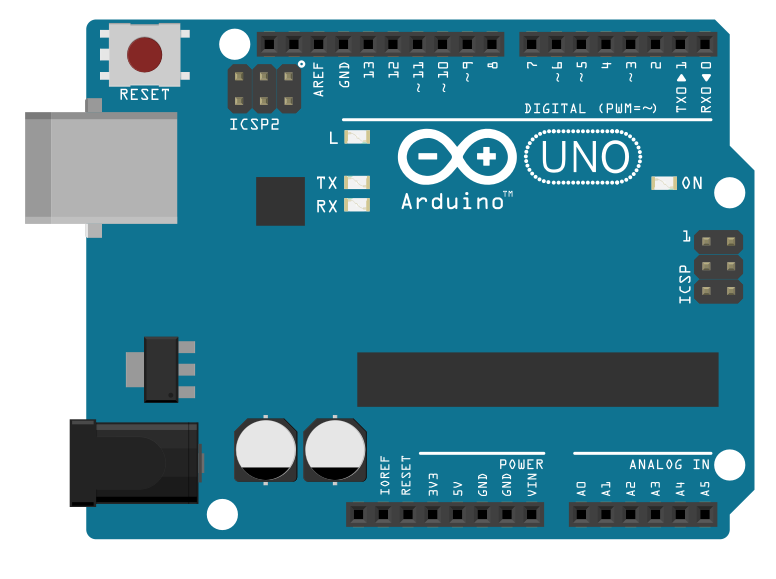
\includegraphics[width=0.7\textwidth]{img/Diagramas/arduinoUno.PNG}
    \caption{Dibujo de Arduino.} \label{Img:Arduino}
\end{figure}



\begin{landscape}
\begin{table}[]
\centering
\resizebox{1.5\textwidth}{!}{%
\begin{tabular}{|l|l|l|l|l|l|l|l|l|l|l|}
\hline
\rowcolor[HTML]{C0C0C0} 
Arduino & PROCESADOR & VOLTAJE OP/IN & MHz CPU & IN/OUT ANALÓGICAS & ENTRADAS/ SALIDAS DIGITALES & EEPROM & SRAM (KB) & FLASH (KB) & USB & UART \\ \hline
Uno & ATmega328P & 5 V / 7-12 V & 16MHz & 6/0 & 14/6 & 1 & 2 & 32 & Regular & 1 \\ \hline
\rowcolor[HTML]{EFEFEF} 
Leonardo & ATmega32U4 & 5 V / 7-12 V & 16MHz & 12/0 & 20/7 & 1 & 2.5 & 32 & Micro & 1 \\ \hline
101 & Intel Curie & 3.3 V/ 7-12V & 32MHz & 6/0 & 14/4 & - & 24 & 196 & Regular & - \\ \hline
\rowcolor[HTML]{EFEFEF} 
Esplora & ATmega32U4 & 5 V / 7-12 V & 16MHz & - & - & 1 & 2.5 & 32 & Micro & - \\ \hline
Arduino Zero & ATSAMD21G18 & 3.3 V / 7-12 V & 48 MHz & 6/1 & 14/10 & - & 32 & 256 & 2 Micro & 2 \\ \hline
\rowcolor[HTML]{EFEFEF} 
Mega 2560 & ATmega2560 & 5 V / 7-12 V & 16 MHz & 16/0 & 54/15 & 4 & 8 & 256 & Regular & 4 \\ \hline
\end{tabular}%
}
\caption{Comparativa Arduinos}
\label{tab:comp_Arduino}
\end{table}
\end{landscape}

\subsection{Decisión sobre SOC}\label{4.DecisionSOC}
Finalmente he determinado que en nuestro proyecto tendremos el control de la instalación domótica desde una Raspberry Pi\cite{misc:RbPWeb}. La justificación se basa en la naturaleza de ambas placas y la necesidad del proyecto: las placas Raspberry Pi están orientadas a utilizarse como un ordenador de poca potencia, mientras que un Arduino está orientado a utilizarse como un equipo electrónico.

Además, se pretende que el proyecto disponga de un Sistema Operativo sobre el que poder programar las funciones que queremos además de poder interactuar con éste de una forma natural además de facilitar el futuro mantenimiento.

Sobre las diferentes Raspberry Pi, podemos observar que prácticamente nos valdría cualquiera para el cometido que le vamos a encargar. En este caso optaré por la Raspberry Pi 2B frente a las demás porque dispongo de una placa en desuso; pero, en caso de tener que escoger una, elegiría una Raspberry Pi 3B+ por su escaso precio y capacidades superiores a la 2B. También deshecharía la 4B por su elevado precio con respecto a la seleccionada y sus problemas de sobrecalentamiento en la penúltima versión ya que al realizar la compra de la misma no dejan elegir la versión de la placa.

\begin{figure}
    \centering
    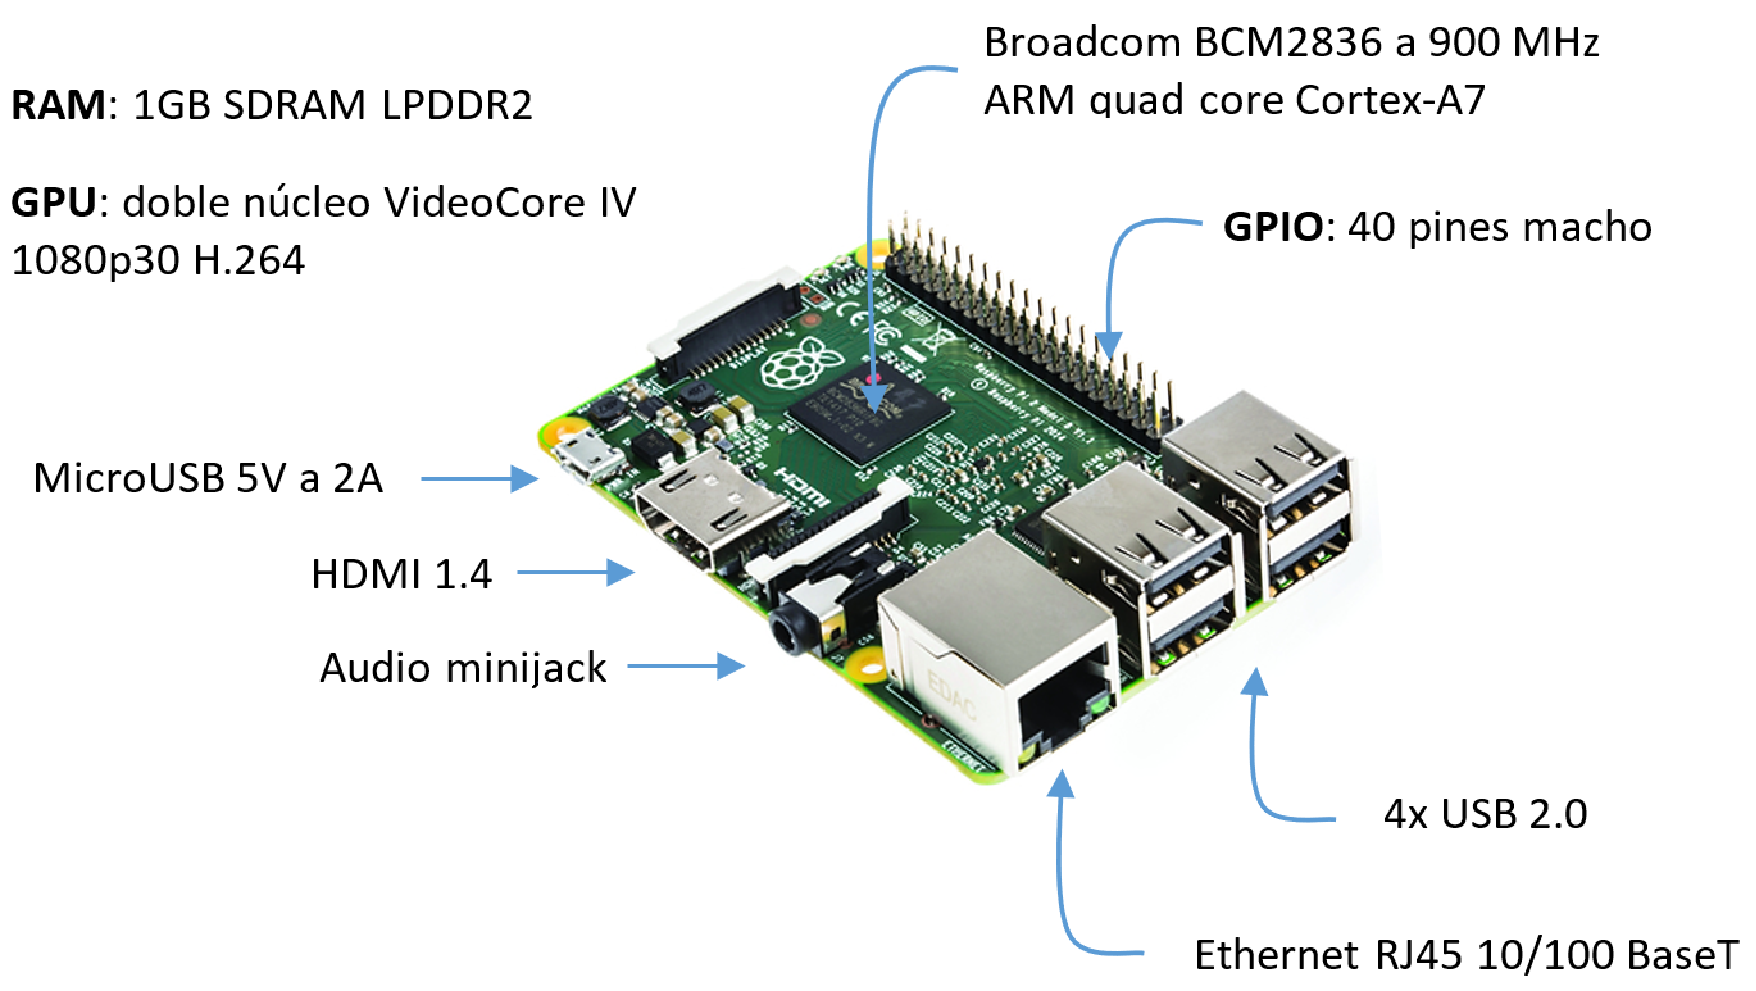
\includegraphics[width=\textwidth]{img/RBP2B.pdf}
    \caption[Especificaciones de Raspberry Pi 2B.]{Especificaciones de Raspberry Pi 2B.}\label{Img:Especificaciones RBP2B}
\end{figure}

\begin{figure}
    \centering
    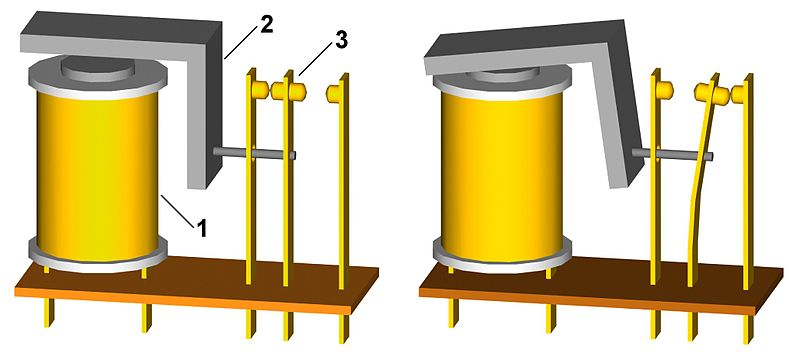
\includegraphics[width=0.7\textwidth]{img/Rele_1.jpg}
    \caption[Estructura interna de un relé]{Estructura interna de un relé.} \label{Img:Rele1}
    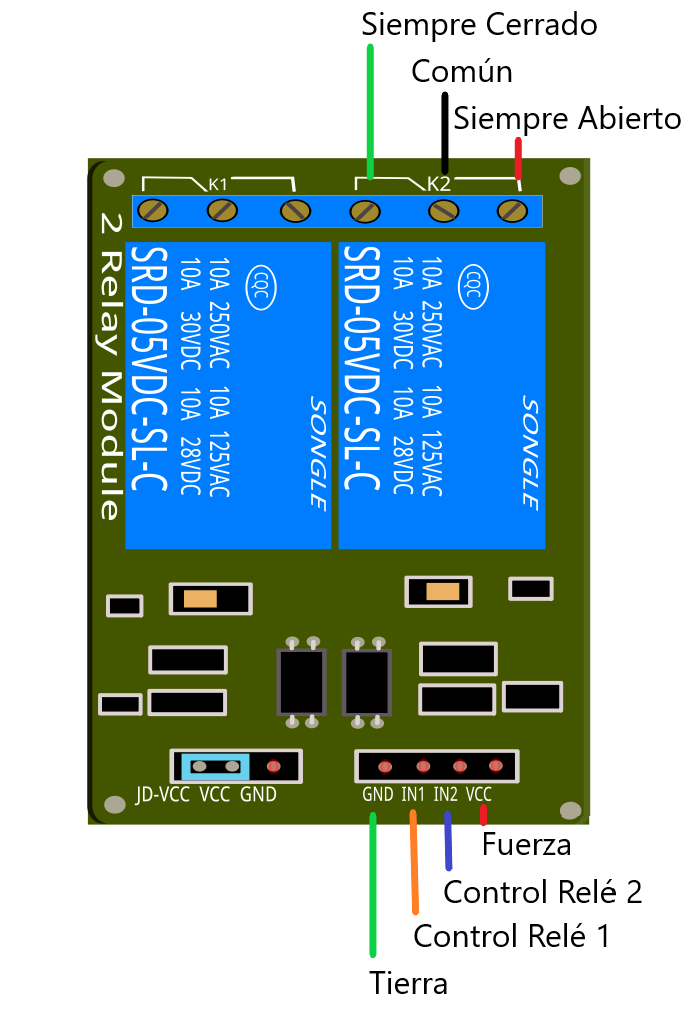
\includegraphics[width=0.4\textwidth]{img/Diagramas/ReleProyecto.png}
    \caption[Diagrama Real Relés del proyecto.]{Diagrama Real Relés del proyecto.} \label{Img:ReleProyecto}
\end{figure}
\subsection{Relé}\label{4:Relé}
Es un dispositivo electromagnético que permite, mediante un circuito primario, abrir o cerrar un circuito secundario. Dicho con otras palabras, desempeña la misma función de un interruptor, es decir, con nuestros relés, dejaremos pasar la energía, o no, a nuestros dispositivos. Podemos ver el funcionamiento interno en la imagen~\ref{Img:Rele1}~\footnote{Imagen original de~\url{https://commons.wikimedia.org/}}. También podemos ver un diagrama, en la imagen~\ref{Img:ReleProyecto}, de como son los relés utilizados en este proyecto con una breve aclaración sobre las conexiones que están a nuestra disposición.



\subsection{Placa de Pruebas o ProtoBoard}\label{4:protoboard}
Es un tablero electrónico para realizar pruebas. Protoboard es la agrupación de los términos ingleses “prototype board”.
Esta protoboard la he configurado para poder hacer fácilmente el interconexionado entre los cables que llegan de los relés y los que van a la Raspberry Pi, evitando posibles tirones y movimiento de cables a la hora de hacer alguna manipulación.

Éstas, disponen de tres zonas diferenciadas(Ver imagen ~\ref{Img:Protoboard}):

\begin{itemize}
    \item \textbf{Canal Central}: Está situada en el medio de la placa, es donde está la zona de las pistas y es donde se colocan los circuitos.
    \item \textbf{Buses}: Se sitúan en los extremos de la placa y disponen de dos líneas:
        \subitem \textbf{Línea roja}: Bus positivo o de voltaje.
        \subitem \textbf{Línea azul}: Bus negativo o de tierra.
    \item \textbf{Pistas}: Existen dos pistas en la zona central de la placa de la imagen y, conducen en sentido contrario de las líneas rojas y azul.
\end{itemize}

\begin{figure}
    \centering
    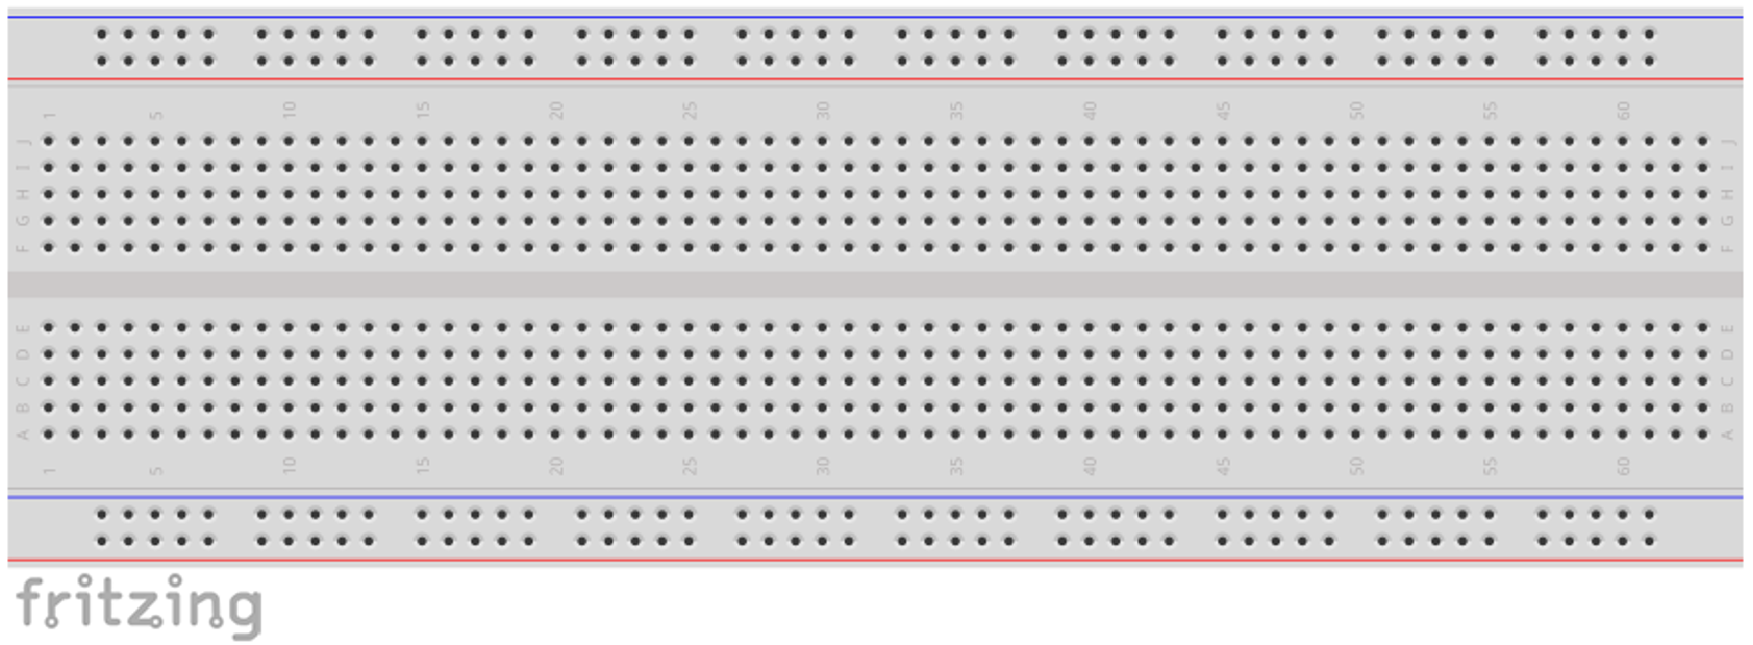
\includegraphics[width=0.9\textwidth]{img/protoboard.pdf}
    \caption{Imagen de una placa <<protoboard>>. } \label{Img:Protoboard}
\end{figure}

\subsection{Router}\label{4:Router}
Es un dispositivo que nos permite interconectar diferentes redes de datos. En mi caso dispongo de un router con WiFi integrado para poder dotar a la Raspberry Pi de salida a Internet.

\section{Plataforma de interacción}\label{4:telegram}
\begin{itemize}
    \item \textbf{Herramientas valoradas:} \href{https://telegram.org/}{Telegram}, \href{https://palletsprojects.com/p/flask/}{Flask}.
    \item \textbf{Herramienta elegida:} \href{https://telegram.org/}{Telegram}.
\end{itemize}
Para finalizar el proyecto con una interfaz de interacción se valoraron las opciones de desarollar un página web ligera o una aplicación de mensajería.
En primer lugar se propuso hacer una aplicación en Flask pero pareció más novedoso y potente hacer un Bot de Telegram de forma que podamos interactuar con él y enviarnos información bajo demanda. Además, se elimina el buscar hosting y dominio para albergar los servicios propios del sistema domótico abaratando más los costes, además de incrementar la seguridad al utilizar mensajería cifrada.

